\documentclass[10pt,a4paper]{article}
\usepackage[utf8]{inputenc}
\usepackage[T1]{fontenc}
\usepackage{amsmath}
\usepackage{amssymb}
\usepackage{graphicx}
\usepackage{hyperref}
\usepackage{multicol}
\usepackage{float}
\graphicspath{{./images/}}
\title{Genes Expression: Alternative Splicing}
\author{R\^{i}mboi Eusebiu - grupa 332}
\begin{document}
	\maketitle
	
	\begin{multicols}{2}
		\section{Genes Expression}
			It's a well known fact that every cell in our body has mostly the same DNA, the differences taking place because of multiple mutations caused by external factors and majority of them being inoffensive. This raises the following important question: how is it possible that 2 cells from different parts of the body can be so distinct? Take for example the comparison between a skin cell and a brain cell: they share mostly the same DNA, but somehow the have so different aspects and can behave so differently that from the outside they seem like totally different structures. The answer resides in a process called \textbf{genes expression}.
			
			When it comes to the actual properties and functions of a certain cell, we must analyze what the proteins it generates, since they are the engines and workers of the cell. Since we know that these polypeptides chains are created through the process of \textbf{proteins synthesis}, the answer is found in the mRNA that is read by ribosomes which form the actual protein chains. More exactly, from the cell DNA to the proteins there are 4 big stages, we will describe below.
			
			Firstly, there is the \textbf{transcription} stage, where the DNA gets copied by the RNA polymerase enzymes into a pre-mRNA form. Then, right after this chain leaves the enzyme, it goes through the \textbf{mRNA processing} (also called post-transcription) stage, where it gets significantly changed by splicing and boundaries additions (5' and 3' sites). In this way, it becomes a mature mRNA and is ready to be sent outside the cell. There, through the process of \textbf{translation} done by ribosomes the mRNA is converted to a protein that is then shipped to fulfill different functions outside and inside the cell.
			
			Along this process, among others, a crucial protein is involved, which is responsible for activation and deactivation of certain genes: \textbf{Transformation Protein (TP)}. This is the main actor that affect what genes reach the ribosome for protein production. Still, given the fact that genes from a DNA are $ \approx $ 20000, most of them not being activated for a particular cell, and also considering the multitude of protein types needed for a single cell to function properly, the human genome evolved a mechanism to fix these issues and, on top of that, to provide a greater translation efficiency.
			
			\begin{figure}[H]
				\centering
				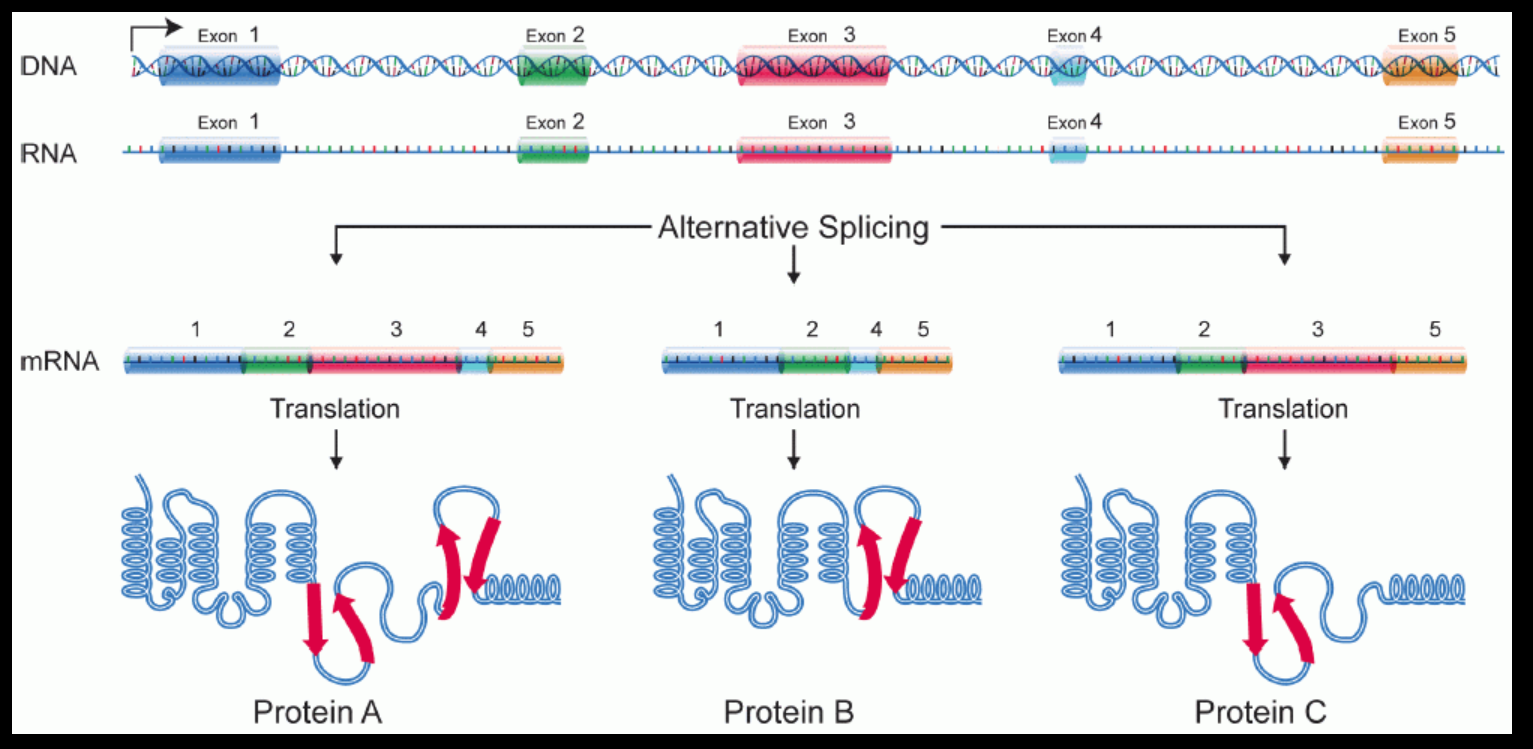
\includegraphics[width=\columnwidth]{proteins_translation.png}
				\caption{\href{https://en.wikipedia.org/wiki/Alternative_splicing}{Proteins Translation based on Alternative Splicing}}
				
			\end{figure}

		\section{Alternative Splicing}
			In its raw form, the pre-mRNA is composed of 2 parts: \textbf{the exons} and \textbf{the introns}. The former is the one that will make it to the mature mRNA string used by ribosomes and the latter represents the part of mRNA which will be removed/spliced. This whole process takes place in the \textbf{post-transcription} phase, and the molecule responsible to execute the procedure is called \textbf{spliceosome}.
			
			Now, the reader may wonder, where does the word \textit{alternative} comes from? Well, it's because the process is not so straightforward as it may seem: the introns are not just simply removed and the resulting string of exons is concatenated (this is called \textbf{constitutive splicing}). Instead, there are multiple variants of this process, called \textit{modes}, by which the mature mRNA is formed. Most of them imply connections between the remaining exons in different orders, thus the name \textit{alternative}. Now, let's explore the most important 4 of them, although you can find up until 6 types in figure \ref{fig:alternative_splicing_modes}:
			\begin{enumerate}
				\item \textbf{Exons skipping}: All introns are removed, but also some of the exons.
				\item \textbf{Intron retention}: There are some introns that are kept in the mature mRNA.
				\item \textbf{Alternative 5' Splice Sites}: The spliceosome chooses a different ending point, taking some codons away from the beginning of the next exon and sticking to the current exon.
				\item \textbf{Alternative 3' Splice Sites}: Same as 5', but mirrored: the spliceosome chooses a different starting point taking a number of codons away from some exon and then appending them to the exon after that.
				\item \textbf{Mutually exclusive exons}: the spliceosome is influenced in such a way it cannot choose some pairs of 2 exons located next to each other.
			\end{enumerate}
		
			How exactly are these splicing patterns chosen depends on many factors, including a large set of protein types synthesized until that point inside the cell, speed of transcription, chromatin structure and much more.
			
			This concludes our short dive into what exactly is the \textit{alternative splicing} and how complex, interconnected and fault tolerant are these genetic processes, which constitute the fundamentals of our very existence.
	
	\end{multicols}

	\begin{figure}[h]
		\centering
		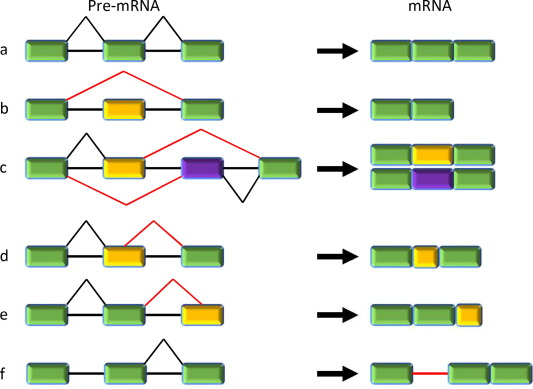
\includegraphics[width=0.8 \textwidth]{modes.jpg}
		\caption{Constitutive and five major types of alternative splicing. a: Constitutive splicing; b: exon skipping (cassette exons); c: mutually exclusive exons; d: alternative 5' splice sites (alternative donors); e: alternative 3' splice sites (alternative acceptors); f: intron retention.}
		\href{https://www.csbj.org/article/S2001-0370%2820%2930534-1/fulltext}{Source}
		\label{fig:alternative_splicing_modes}
	\end{figure}

	\section*{Bibliography}
		\begin{itemize}
			\item \href{https://en.wikipedia.org/wiki/Alternative_splicing}{Wikipedia - Alternative Splicing}
			\item \href{https://eu.idtdna.com/page/support-and-education/decoded-plus/what-is-alternative-splicing-and-why-is-it-important/}{IDT - What is alternative splicing and why is it important?}
			\item \href{https://www.nature.com/articles/s41580-022-00545-z}{Nature Journal - The physiology of alternative splicing}
			\item \href{https://en.wikipedia.org/wiki/Protein_biosynthesis}{Wikipedia - Proteins Biosynthesis}
			\item \href{https://pmc.ncbi.nlm.nih.gov/articles/PMC4360811/}{National Library of Medicine Journal}
		\end{itemize}
	
\end{document}